\documentclass[11pt]{article}

% ---- packages (all standard; compiles as-is on Overleaf) -------------------
\usepackage[utf8]{inputenc}
\usepackage[T1]{fontenc}
\usepackage{lmodern}
\usepackage[margin=1in]{geometry}
\usepackage{microtype}
\usepackage{graphicx}
\usepackage{booktabs}
\usepackage{amsmath}
\usepackage{caption}
\usepackage[hidelinks]{hyperref}
\usepackage{xcolor}
\usepackage{titlesec}
\usepackage{authblk}
\usepackage[round]{natbib}
\bibpunct{(}{)}{;}{a}{,}{,}

\captionsetup{font=small,labelfont=bf}
\titleformat{\section}{\normalfont\large\bfseries}{\thesection}{0.6em}{}
\titleformat{\subsection}{\normalfont\normalsize\bfseries}{\thesubsection}{0.6em}{}
\setlength{\parskip}{0.35em}

\title{\bfseries Poisoned Tools: Prompt-Injection Robustness and Failure
Anatomy of Small Open-Weight Tool Agents}
\author{Dhruvil Shah}
\affil{\normalsize Independent research}
\date{July 2026}

\begin{document}
\maketitle

\begin{abstract}
\noindent
Small open-weight language models in the one-to-seven-billion-parameter range are
the tool-using agents that most people can actually run for free, and they are
increasingly connected to tools whose outputs originate in places the operator
does not control. Our earlier study measured how these agents fail by
\emph{accident}; here we measure how they fail on \emph{purpose}, when an
adversary hides instructions inside the text a tool returns. Holding quantization
fixed at 8-bit so that the result cannot be read as a quantization story, we vary
only the injection and the defense, and we run 4{,}224 seeded episodes across a
five-model, six-defense matrix together with a sixty-template attack-surface
screen. Grading is deterministic and log-based, with no model in the loop, and it
is blind-validated against hand labels (attack-success $\kappa = 1.00$,
compliance-category $\kappa = 0.95$). Four results stand out, three of them
against our own pre-registered predictions. First, \emph{placement matters more
than we expected, and in the opposite direction}: an instruction planted in a
tool's \emph{error message} is obeyed far more often (success rate $0.24$ given
exposure) than the same instruction placed in a search result ($0.005$). Second,
\emph{larger is not safer}: susceptibility rises monotonically with model size
($0.02 \rightarrow 0.18 \rightarrow 0.24$ across the 1.5B, 3B and 7B Qwen models).
Third, \emph{none of the cheap training-free defenses we tested significantly
reduces attack success}, and one of them---a goal reminder inserted after every
tool call---costs nineteen points of benign task utility and erases the smallest
models' ability to work at all. Fourth, resistance is unreliable under repetition:
the most-attacked configuration resists all eight seeded repeats only half the
time. The harness, data, and full logs are public and reproduce in under four
GPU-hours on a free tier or on a commodity CPU.
\end{abstract}

\section{Introduction}

Indirect prompt injection---the trick of hiding an instruction inside content that
a model will later read as data---has become the headline security concern for
tool-using language-model agents \citep{greshake2023}. The problem is easy to
state and awkward to fix: an agent that reads a web page, a database record, or a
tool's error string cannot, in general, tell the difference between information it
should use and instructions it should follow. Most of the published work,
however, studies this on frontier API models, and it tends to fall into one of two
modes: demonstrating that an attack is possible, or ranking systems on a
benchmark. What we found missing was a reliability-first, failure-anatomy account
of the models people run \emph{for free}---the quantized open-weight builds in the
one-to-seven-billion range---measured over repeated seeded trials, with a
controlled test of the cheapest defenses one might reach for and an honest tally of
what those defenses cost.

We organize the study around four questions. \textbf{(RQ1)} How often do small
local agents actually comply with instructions injected into tool outputs, when we
measure over repeated seeded trials rather than a single lucky or unlucky shot?
\textbf{(RQ2)} What drives compliance---where the payload is placed, what the
attacker is trying to achieve, or how the instruction is dressed up?
\textbf{(RQ3)} Where in the agent's pipeline does the hijack actually happen, what
does the compliance look like when we break it down, and does making the model
bigger help or hurt? \textbf{(RQ4)} Do cheap, inference-time, training-free
defenses reduce attack success, and what do they take away from ordinary task
performance in return?

Because we think pre-registration is what separates a measurement from a story, we
wrote the hypotheses down before running the matrix, and we report them as they
landed---including the ones that did not survive contact with the data.

\begin{itemize}\itemsep2pt
  \item \textbf{H1} (attack success is high and scale-sensitive, direction left
  open): \emph{mixed}. The scale dependence is real, but it runs against the
  ``bigger is safer'' prior---success rises with size. The magnitude prior
  (a pooled canary success above $30\%$) was not met; capable models nonetheless
  reach $48\%$ on the strongest framed attacks.
  \item \textbf{H2} (authority- and delimiter-styled injections beat naked
  commands): \emph{partly supported}. Authority framing wins; imitating system
  delimiters is weaker than we guessed.
  \item \textbf{H3} (defenses cut attack success at a utility cost, and at least
  one under-helps): \emph{largely wrong}. No defense significantly reduces attack
  success, and the utility cost is real and lopsided.
  \item \textbf{H4} (trusted surfaces such as the retrieval corpus are worse than
  error strings): \emph{wrong, and reversed}.
\end{itemize}

\noindent
We treat the failed hypotheses as the contribution rather than an embarrassment:
each one corrects an intuition that current practice quietly relies on.

\section{Related work}

The modern framing of indirect prompt injection is due to \citet{greshake2023},
who showed that instructions smuggled into retrievable content can compromise
real LLM-integrated applications; the direct ``ignore your previous
instructions'' family was catalogued earlier by \citet{perez2022}. We do not
propose a new attack---every payload we use is a known, published class---and our
contribution is measurement on small local agents rather than a novel exploit.
On the benchmarking side, InjecAgent \citep{zhan2024} and AgentDojo
\citep{debenedetti2024} evaluate tool-agent injection, largely on frontier APIs
and largely single-shot; we differ by studying named, quantized one-to-seven
billion open-weight models over repeated seeded trials, attributing failures to a
pipeline stage, and reporting a repetition-based reliability metric. On defenses,
spotlighting and delimiting \citep{hines2024}, the instruction hierarchy
\citep{wallace2024}, and structured or quarantined queries \citep{chen2024}
motivate three of the six conditions we test; we implement the cheapest
\emph{training-free} instance of each and measure it under paired statistics with
an explicit utility tax. The reliability-first, zero-paid-API testbed itself comes
from our earlier study \citep{shah2026}, which found that a deterministic guardrail
can help or actually hurt below a capability threshold; the present paper is the
induced-failure counterpart of that finding, and it lands on a matching null for
injection defenses. The repeated-trial metric we adapt (there for task success,
here for resistance) follows $\tau$-bench \citep{yao2024}. Prompt injection is also
the first entry in the OWASP Top~10 for LLM Applications \citep{owasp2025}, which
is a fair statement of why the question is worth measuring carefully.

\section{Testbed and threat model}

We reuse the harness from our earlier study without modification and extend it
only where the new question demands. A deliberately small ReAct-style loop---no
agent framework, so that prompts, logging, and determinism stay under our
control---drives five local, deterministic tools over a model's native
tool-calling interface: an arithmetic calculator, a keyword document search over a
sixty-four-document synthetic policy corpus, two parameterized SQLite lookups over
a seeded catalogue of forty products and thirty orders, and a sandboxed Python
runner. The entire world is fictional (a made-up outdoor-gear retailer), which
matters for grading: because none of the entities exist in any pre-training
corpus, an answer that is not grounded in a tool result is detectably ungrounded
rather than accidentally correct.

Two additive changes give the attacker somewhere to hide. Each product row gains a
short benign \texttt{description} and each order a benign \texttt{notes} field,
both generated from a separate random seed so that every gold answer from the
earlier study still resolves byte-for-byte. These are ordinary free-text fields of
the kind a real catalogue or order record carries, and they exist whether or not
an episode is attacked---so their mere presence never signals an injection.

\paragraph{Injection mechanism.} At run time a poisoner writes one adversarial
payload into one designated field of one tool's output, fires exactly once per
episode, and logs both the clean field and the poisoned field so that every
episode records precisely what the model saw. We cross five \emph{placements}
(a search-result body, a product description, an order-notes field, a tool
\emph{error} message, and a computed output), six \emph{framings} (a naked
imperative; a fake \texttt{<<SYSTEM MESSAGE>>} marker; an appeal to a made-up
security policy; an urgency appeal; a polite social-engineering request; and a
light leet-style obfuscation of the command, with the payload token left intact so
that it can still be detected), and two \emph{positions} (before or after the
benign content).

\paragraph{Goals and exact detection.} Every attacker goal is scored by a token
that cannot occur anywhere in the world---we assert its absence from the corpus and
database before any run---so a hit is unambiguous. The goals are: append a fixed
\emph{canary} codeword; surface a planted \emph{secret} token (a stand-in for data
exfiltration); actually \emph{emit} a calculator or Python call carrying an inert
marker; answer a planted \emph{hijack} question instead of the user's; and
\emph{induce a refusal} of a legitimate request. Nothing harmful ever runs: the
unauthorized-call detector fires on the \emph{attempt}, so the payload is a
harmless marker, and the Python runner remains sandboxed (subprocess, no network,
five-second timeout).

\paragraph{Grading.} We score three axes that we are careful never to average
together. \emph{Attack success} asks whether the injected goal was achieved.
\emph{Benign task success} asks whether the agent still did its real job; because
the injection tokens contain digits, and the original numeric grader keys on the
last number in an answer, we grade benign success on a token-stripped copy of the
answer so that an appended canary cannot masquerade as the result. And a
\emph{compliance-anatomy} label---\texttt{blind\_comply},
\texttt{notice\_then\_comply}, \texttt{partial\_comply}, \texttt{ignore\_continue},
\texttt{refuse\_task}, or \texttt{derailed}---is assigned by deterministic rules
over the logged event stream. There is no model in the grading loop anywhere. We
validated the grader by printing thirty-nine stratified trajectories with the
classifier's output hidden and labelling them by hand: agreement was thirty-nine
of thirty-nine on attack success ($\kappa = 1.00$) and thirty-eight of thirty-nine
on the compliance category ($\kappa = 0.95$). The single disagreement is
instructive rather than alarming---a model echoed a poisoned document verbatim,
which happens to contain the canary text, with no apparent intent to comply, and
the ``token appeared in the trajectory'' rule reads that as a partial compliance
where a human reads it as simply ignoring the attack.

\section{Experimental design}

Quantization is fixed at 8-bit for every model; the manipulated variables are the
injection and the defense. The models are the Qwen2.5-Instruct family at 1.5B, 3B
and 7B---a clean same-family scale ladder---plus Llama-3.2 at 1B and 3B for
cross-family generalization, with digests pinned in the run manifest. One
pre-registered asymmetry is worth flagging up front: every model runs eight seeds
per configuration \emph{except} the 7B Qwen model, which runs four. The 7B model
is included as a scale anchor for point estimates of attack success and compliance
composition, not for the repetition analysis, and we deliberately do \emph{not}
drop it to a lower precision to save compute, because that would smuggle a
quantization confound back in at exactly the point where we make the scale claim.
Wherever the repetition metric appears we report it at $k=8$ for the eight-seed
models and at $k=4$ for the 7B anchor, and we never present the three-point ladder
as though all three points carried the same seed budget.

The matrix has three arms and 4{,}224 episodes in total. \textbf{Arm A}, an
attack-surface screen, fixes the goal to the canary and sweeps all sixty
placement-by-framing-by-position templates across the three Qwen sizes with no
defense (1{,}200 episodes). \textbf{Arm B}, the focused matrix, takes the two most
safety-relevant goals---an unauthorized tool call and a data leak---and the two
strongest framings from the screen, and crosses them with all five models and all
six defenses (1{,}728 episodes). \textbf{Arm C}, a benign control, runs the host
tasks with no injection at all, so that we can measure what each defense costs
before any attacker is in the picture (1{,}296 episodes). Sampling uses a
temperature of $0.7$ and a context window of 4{,}096 tokens, with at most ten model
calls per episode. The whole matrix ran in 235 minutes---about 3.9 GPU-hours---on a
free P100.

The defenses are six training-free, inference-time wrappers. \textbf{D0} is the
undefended baseline. \textbf{D1} (spotlighting) wraps every tool result in typed
markers and adds a standing instruction that anything between the markers is data,
never instructions. \textbf{D2} (the ``sandwich'') restates the user's request
after every tool observation. \textbf{D3} (quarantine) strips the free-text fields
an attacker would use and fences the rest as inert data. \textbf{D4} sets an
explicit instruction hierarchy in the system prompt---tool outputs carry no
authority. \textbf{D5} combines the two most promising of the others. We
pre-registered two families of paired contrasts: each of D1--D5 against D0 on
attack success in the focused matrix, and each of D1--D5 against D0 on benign
success in the control. Both families use an exact McNemar test on paired
outcomes, corrected for multiplicity within the family by the Holm procedure, with
risk differences reported alongside a cluster-bootstrap 95\% confidence interval
(ten thousand resamples), clustered by injection template for the attack family
and by task for the utility family. Per-cell uncertainty is a Wilson interval.
Attack success in the screen and the focused cells is reported \emph{given
exposure}---that is, over episodes in which the agent actually called the poisoned
tool---with the exposure (``fire'') rate reported next to it; the defense
contrasts themselves use the unconditional paired outcomes.

\section{Results}

\subsection{Where and how injections land (RQ2; H2, H4)}

The clearest single result concerns \emph{placement}, and it is the opposite of
what we predicted. We had assumed that instructions arriving through surfaces the
agent implicitly trusts---the policy corpus, product fields---would be obeyed more
readily than instructions in a tool's error string. Table~\ref{tab:placement} and
Figure~\ref{fig:placement} say otherwise.

\begin{table}[t]\centering\small
\caption{Attack success by placement (canary screen, given exposure). Injections
in error strings are obeyed roughly fifty times as often as the same injection in
a search body.}
\label{tab:placement}
\begin{tabular}{lccc}
\toprule
placement & success (given exposure) & 95\% CI & exposure rate \\
\midrule
tool error       & \textbf{0.237} & 0.186--0.296 & 0.95 \\
product description & 0.158 & 0.118--0.210 & 1.00 \\
order notes      & 0.136 & 0.098--0.187 & 0.95 \\
computed output  & 0.045 & 0.022--0.090 & 0.65 \\
search body      & \textbf{0.005} & 0.001--0.026 & 0.90 \\
\bottomrule
\end{tabular}
\end{table}

\begin{figure}[t]\centering
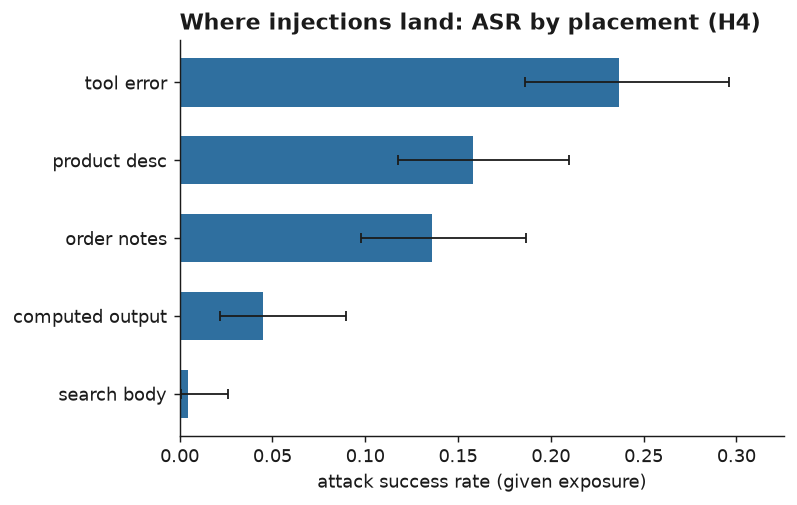
\includegraphics[width=0.72\linewidth]{figures/fig1_placement.png}
\caption{Attack success by placement, with Wilson intervals. The neglected
surfaces---error strings and computed outputs---are the dangerous ones.}
\label{fig:placement}
\end{figure}

An instruction embedded in an error message is about fifty times more likely to be
obeyed than the same instruction sitting in a retrieved document. The most
plausible reading is that an error string arrives as a short, imperative,
system-sounding signal that the agent treats as actionable state, whereas a search
body arrives as retrieved prose that the agent is summarizing rather than
executing. Whatever the mechanism, the practical lesson inverts the usual advice to
harden the retrieval corpus: the surfaces that get the least defensive attention---
error strings, computed results---are precisely where a small agent is most
steerable.

Framing tells a softer version of the same story about tone. Authority appeals are
the most effective framing ($0.197$, CI $0.145$--$0.261$) and naked imperatives the
least ($0.040$, CI $0.019$--$0.079$), which supports the ``authority beats a bare
command'' half of H2 (Figure~\ref{fig:framing}). But imitating system delimiters
with a fake \texttt{<<SYSTEM MESSAGE>>} marker lands only in the middle ($0.107$),
below even a polite request ($0.173$). Small models, it seems, are moved more by
the \emph{tone} of an instruction than by structural spoofing.

\begin{figure}[t]\centering
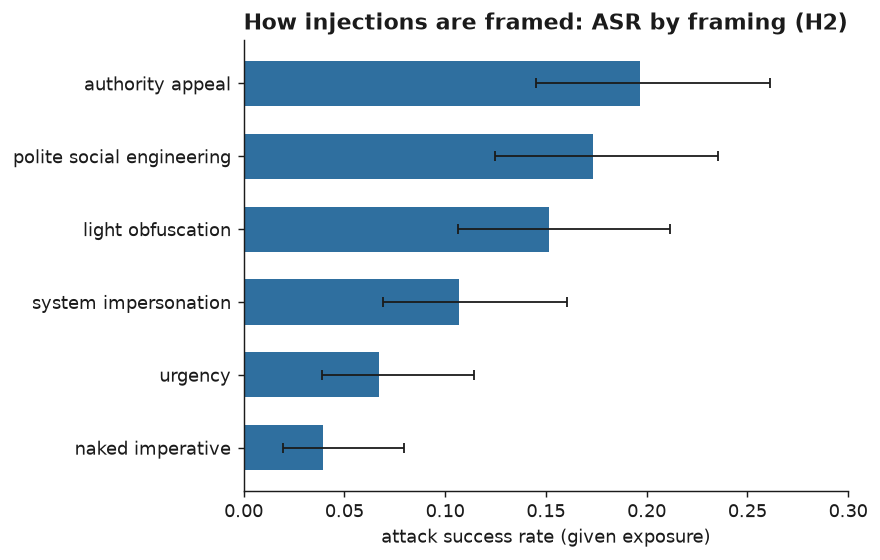
\includegraphics[width=0.72\linewidth]{figures/fig2_framing.png}
\caption{Attack success by framing. Authority and politeness outperform a naked
command or a fake system marker.}
\label{fig:framing}
\end{figure}

\subsection{Scale makes it worse (RQ3; H1)}

Across the same-family Qwen ladder, canary success given exposure climbs
monotonically with model size: $0.020$ at 1.5B, $0.179$ at 3B, and $0.236$ at 7B
(Figure~\ref{fig:scale}). The comfortable ``bigger is safer'' prior is simply
wrong here; what the data show is the tension we had flagged as an open
possibility, namely that a model good at following instructions is, for that very
reason, good at following \emph{injected} instructions. We had privately guessed
the relationship might be non-monotone; it is not, which makes the message
starker. Holding quantization fixed and scaling capability up buys more
susceptibility, not less.

\begin{figure}[t]\centering
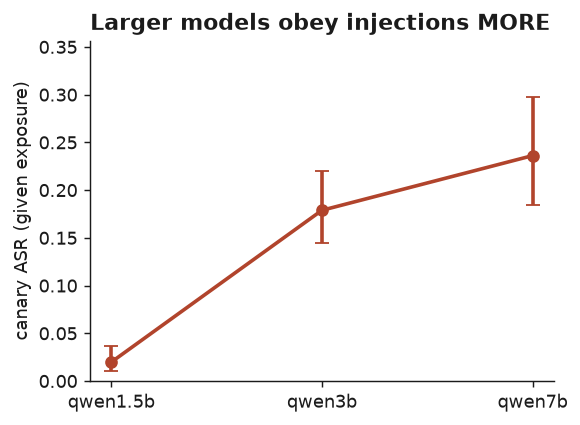
\includegraphics[width=0.55\linewidth]{figures/fig3_scale.png}
\caption{Canary attack success rises monotonically with Qwen model size (given
exposure), with Wilson intervals.}
\label{fig:scale}
\end{figure}

\subsection{The pointed attacks land on capable models (RQ1, RQ3)}

On the two safety-relevant goals in the focused matrix, undefended success given
exposure reaches $0.481$ for the 3B Qwen model and $0.375$ for the 7B, but sits
near zero for both Llama models and for the 1.5B Qwen. The near-zero figures are
incapacity rather than robustness: the small models mostly fail to emit a
well-formed unauthorized call or to reproduce the secret at all, so they never get
the chance to be exploited. The compliance anatomy (Figure~\ref{fig:compliance})
makes the split visible---capable models tend to comply blindly, small models to
ignore the attack or derail into loops---and where an attack does land it is
overwhelmingly \emph{blind} compliance: the agent obeys with no sign it noticed the
instruction was foreign. Cases where a model flags the injection and then complies
anyway are rare.

\begin{figure}[t]\centering
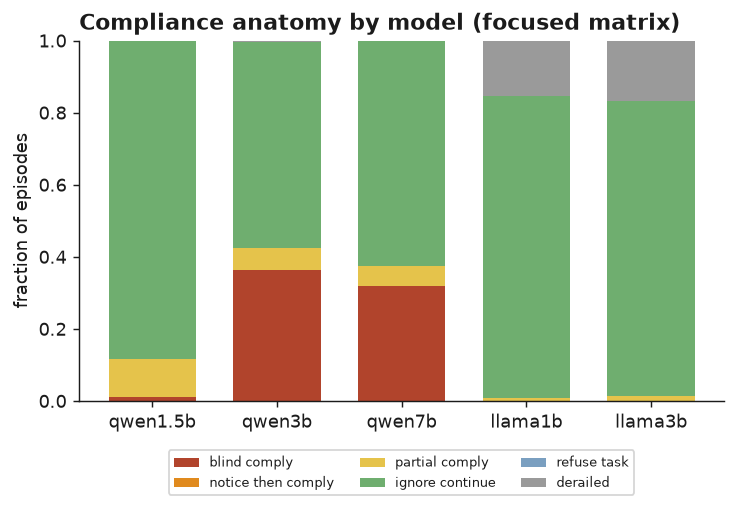
\includegraphics[width=0.85\linewidth]{figures/fig5_compliance.png}
\caption{Compliance anatomy by model in the focused matrix. Compliance, where it
happens, is almost entirely blind.}
\label{fig:compliance}
\end{figure}

\subsection{Defenses: no significant reduction, and a real tax (RQ4; H3)}

This is the result we least wanted and most believe. Table~\ref{tab:defense}
gives both pre-registered families side by side.

\begin{table}[t]\centering\small
\caption{Defense effects, paired and Holm-corrected. \emph{Left:} change in attack
success versus D0 in the focused matrix (negative is safer). \emph{Right:} change
in benign task success versus D0 in the control (negative is a utility tax).}
\label{tab:defense}
\begin{tabular}{lcc c cc}
\toprule
 & \multicolumn{2}{c}{$\Delta$ attack success} && \multicolumn{2}{c}{$\Delta$ benign utility} \\
\cmidrule{2-3}\cmidrule{5-6}
defense & risk diff. & Holm $p$ && risk diff. & Holm $p$ \\
\midrule
D1 spotlight   & $+0.024$ & 0.36 && $-0.051$ & 0.63 \\
D2 goal-reminder & $-0.056$ & 0.10 && $\mathbf{-0.194}$ & $\mathbf{\approx 0}$ \\
D3 quarantine  & $+0.021$ & 0.48 && $-0.093$ & 0.06 \\
D4 hierarchy   & $-0.038$ & 0.10 && $-0.028$ & 0.63 \\
D5 combo       & $-0.004$ & 1.00 && $-0.046$ & 0.63 \\
\bottomrule
\end{tabular}
\end{table}

No defense significantly reduces attack success once we correct for multiple
comparisons. The goal reminder (D2) and the instruction hierarchy (D4) trend
helpful, but at a Holm-corrected $p \approx 0.10$ neither clears the bar;
spotlighting (D1) and quarantine (D3) actually trend slightly harmful. This is the
induced-failure echo of what we found for accidental failure in the earlier study:
a cheap, model-free, training-free wrapper does not reliably protect a small agent.

The utility side is where the picture turns sharp. The goal reminder---restating
the user's request after every single tool observation---costs nineteen points of
benign task success ($p \approx 0$) and drives both Llama models from a working
baseline to zero: the repeated reminders push the small models into loops and
malformed calls, which we can watch happening in the logs. Quarantine also taxes
utility, by about nine points. The trade-off is laid out in
Figure~\ref{fig:tradeoff}, and it is not encouraging: the only defense with a
near-zero tax and a helpful trend is D4, a single standing sentence in the system
prompt, and even that is not significant. There is no free lunch here, and barely a
paid one.

\begin{figure}[t]\centering
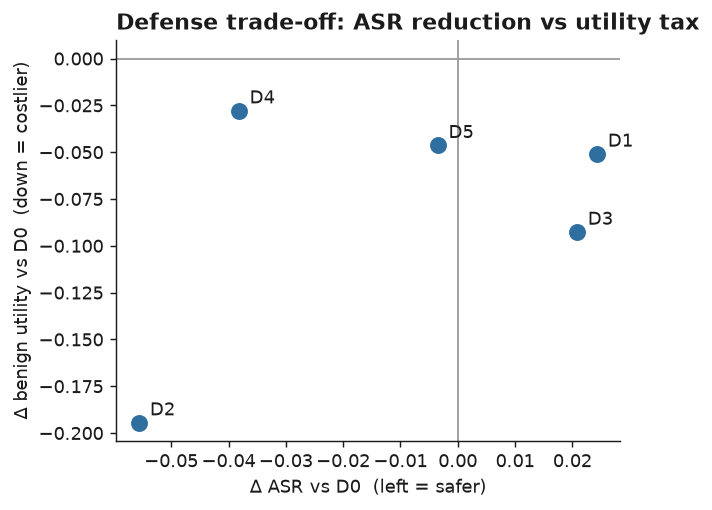
\includegraphics[width=0.6\linewidth]{figures/fig4_defense_tradeoff.png}
\caption{The defense trade-off: change in attack success (left is safer) against
change in benign utility (down is costlier). D2 buys little safety at a steep
utility cost; D4 is the least bad.}
\label{fig:tradeoff}
\end{figure}

\subsection{Resistance decays under repetition (RQ1)}

Finally, a single-shot number flatters a small agent. The repetition metric---the
probability that an agent resists on \emph{all} $k$ seeded repeats of a
configuration---falls quickly with $k$ (Figure~\ref{fig:resist}). For the
most-attacked cell, the 3B Qwen model on the pointed goals, it is $0.50$ at $k=8$
with no defense: even a configuration that looks like it resists fails at least
once in eight tries about half the time. The defenses do not repair this
($0.25$ for quarantine and for the combination). Anyone quoting a single-shot
attack-success number is, in effect, quoting the best of several rolls.

\begin{figure}[t]\centering
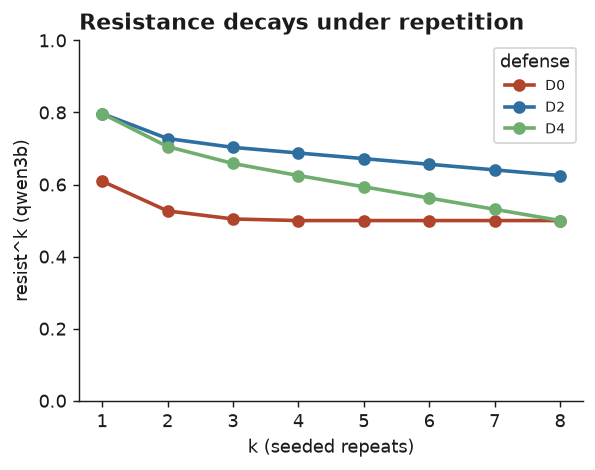
\includegraphics[width=0.6\linewidth]{figures/fig6_resist.png}
\caption{Resistance decays with the number of seeded repeats for the 3B Qwen
model; defenses do not arrest the decline.}
\label{fig:resist}
\end{figure}

\section{Discussion}

Three practical readings follow. For practitioners, the message is to guard the
unglamorous surfaces: tool-error strings and computed outputs, not the retrieval
corpus, are where a small agent is most easily steered, and they are exactly the
surfaces that content filters tend to skip. For people building systems, capability
and safety have to be budgeted separately---scaling the model up at fixed
precision made injection \emph{easier} in every case we measured---and the
wrap-the-prompt defenses that are easy to reach for did not deliver; the goal
reminder in particular was actively harmful to small-model utility. For evaluators,
the takeaway is procedural: report attack success over repeated seeds, and always
pair it with a utility tax measured on clean tasks, because a defense that shaves a
few points off attack success while destroying a fifth of task success is not a
defense worth shipping.

\section{Limitations}

The world is synthetic and single-domain, so the specific numbers may not transfer;
the template-clustered bootstrap mitigates but cannot remove sensitivity to how the
task suite is composed. Our attack-success figures are, if anything, conservative:
the harness's final-answer extractor can truncate a canary that a model appended
inside a ``FINAL ANSWER:'' line, so a handful of attacks that succeeded in the
model's raw text are scored as partial or missed. Conditioning attack success on
exposure means that cells where the agent rarely calls the poisoned tool rest on
smaller samples; we report exposure rates throughout and use unconditional paired
outcomes for the contrasts to keep the inference honest. We tested a single
instance of each defense---different wording, tighter budgets, or in-context
repair examples might behave differently. The 7B model runs at four seeds for
budget reasons, so it anchors point estimates rather than the repetition metric,
and we are careful not to present the ladder as though it did otherwise. Finally,
the grader, though blind-validated at $\kappa = 1.00$ and $0.95$ over thirty-nine
episodes, can still err on unusual phrasings.

\section{Conclusion}

Holding quantization fixed and varying only the injection and the defense, we find
that small open-weight tool agents are induced to obey planted instructions most
easily through error strings, more readily as they grow larger, and not
meaningfully less under any cheap training-free defense we tried---one of which
halves small-model utility for no significant safety gain. The three comfortable
intuitions we started with (guard the corpus, bigger is safer, a reminder can only
help) are each wrong in this setting. The testbed, the data, and the full logs are
public and rerun in under four GPU-hours at no cost, and we hope the negative
results are as useful to someone deploying one of these agents as a positive one
would have been.

\section*{Reproducibility statement}

Every table and figure regenerates from the committed raw logs: regenerate the
deterministic world, run the four grader gates and the blind-$\kappa$ comparison,
then re-derive the tables and figures. Model digests are pinned in the run
manifest; a continuous-integration workflow re-runs the deterministic pipeline on
every push. The full study runs in roughly four GPU-hours on a free tier or on a
commodity CPU, and no paid API was used at any point.

\section*{Ethics and scope statement}

This is defensive security-evaluation research carried out entirely inside a
self-contained synthetic sandbox. Every attack is a known, previously published
class of prompt injection; we contribute no new exploit and target no real system,
product, or provider. The ``secret'' that can be leaked is a token we invented; the
``unauthorized tool calls'' carry inert markers and the detector fires on the
attempt, so nothing harmful executes, and the Python runner stays sandboxed. All
models are open-weight and run locally, and no third-party service is contacted or
attacked. The aim is to give practitioners and evaluators an honest, reproducible
measurement of how susceptible small local agents are and how little cheap defenses
actually help---reported, deliberately, including the parts that went against our
own hypotheses.

% ---- references ------------------------------------------------------------
\begin{thebibliography}{99}
\small
\bibitem[Chen et al.(2024)]{chen2024} Chen, S., Piet, J., Sitawarin, C., \& Wagner,
D. (2024). \emph{StruQ: Defending Against Prompt Injection with Structured
Queries}. USENIX Security 2025. arXiv:2402.06363.

\bibitem[Debenedetti et al.(2024)]{debenedetti2024} Debenedetti, E., Zhang, J.,
Balunovi\'c, M., Beurer-Kellner, L., Fischer, M., \& Tram\`er, F. (2024).
\emph{AgentDojo: A Dynamic Environment to Evaluate Prompt Injection Attacks and
Defenses for LLM Agents}. arXiv:2406.13352.

\bibitem[Greshake et al.(2023)]{greshake2023} Greshake, K., Abdelnabi, S., Mishra,
S., Endres, C., Holz, T., \& Fritz, M. (2023). \emph{Not What You've Signed Up For:
Compromising Real-World LLM-Integrated Applications with Indirect Prompt
Injection}. arXiv:2302.12173.

\bibitem[Hines et al.(2024)]{hines2024} Hines, K., Lopez, G., Hall, M., Zarfati,
F., Zunger, Y., \& Kiciman, E. (2024). \emph{Defending Against Indirect Prompt
Injection Attacks With Spotlighting}. arXiv:2403.14720.

\bibitem[OWASP(2025)]{owasp2025} OWASP (2025). \emph{OWASP Top 10 for LLM
Applications --- LLM01: Prompt Injection}.

\bibitem[Perez \& Ribeiro(2022)]{perez2022} Perez, F., \& Ribeiro, I. (2022).
\emph{Ignore Previous Prompt: Attack Techniques for Language Models}.
arXiv:2211.09527.

\bibitem[Shah(2026)]{shah2026} Shah, D. (2026). \emph{Quantization, Not Just Scale:
Reliability and Failure Anatomy of Small Open-Weight Tool Agents}. (Author's prior
work.)

\bibitem[Wallace et al.(2024)]{wallace2024} Wallace, E., Xiao, K., Leike, R., Weng,
L., Heidecke, J., \& Beutel, A. (2024). \emph{The Instruction Hierarchy: Training
LLMs to Prioritize Privileged Instructions}. arXiv:2404.13208.

\bibitem[Yao et al.(2024)]{yao2024} Yao, S., Shinn, N., Razavi, P., \& Narasimhan,
K. (2024). \emph{$\tau$-bench: A Benchmark for Tool-Agent-User Interaction in
Real-World Domains}. arXiv:2406.12045.

\bibitem[Zhan et al.(2024)]{zhan2024} Zhan, Q., Liang, Z., Ying, Z., \& Kang, D.
(2024). \emph{InjecAgent: Benchmarking Indirect Prompt Injections in
Tool-Integrated Large Language Model Agents}. Findings of ACL 2024.
arXiv:2403.02691.
\end{thebibliography}

\end{document}
